% Introduction

\section{Scope of this study}

Firms are finding it harder to compete in the knowledge-based economy. They can no longer rely solely on their internal knowledge-base to remain competitive. Not surprisingly, a growing number of firms are embracing open innovation as a competitive strategy. Not only does this allow them to access external knowledge resources, it also enables them to profit from internally developed knowledge by making it available to other firms \citep{laursen2006open,chesbrough2013managing,stanko2017under}. Despite mounting evidence on the potential benefits of open innovation, little is known about knowledge sharing practices in open innovation \citep{lakemond2016match}. This study attempts to fill this gap by examining the individual, organisational, and managerial antecedents of knowledge sharing in three open innovation projects. Particular attention is given to tacit knowledge sharing, a vital ingredient for successful innovation \citep{leonard1998role,koskinen2002role,cavusgil2003tacit,seidler2008use,leonard2014knowledge}.

\section{Background}

\subsection{Defining innovation}

Innovation may be defined as \enquote{the development and implementation of new ideas by people who, over time, engage in relationships with others within an institutional and environmental context} \citep[][pg.]{van1986central}. So long as an idea is perceived as new to the people involved, it is an innovation even though others may see it as nothing more than an imitation of something that exists elsewhere \citep{van1986central}. Innovation is essentially about renewing the business so it can enhance its ability to create value and remain competitive \citep{schumpeter1950capitalism}. Failure to innovate places a firm's ability to survive and prosper at risk \citep{bessant2005managing}. \medskip

\subsection{Trend towards open innovation}

The ever-increasing technical complexity of products, processes, and services demands levels of knowledge beyond what most firms possess or can develop in a market-relevant time-frame. Many firms are turning to open innovation as a competitive strategy \citep{enkel2009open,bessant2013innovation}. Open innovation is formally defined as a distributed innovation process based on carefully managed knowledge flows across firm boundaries using mechanisms as per the firm's business model\footnote{The term \enquote{business model} is defined as \enquote{the chosen system of inputs, business activities, outputs and outcomes that aims to create value over the short, medium, and long term} \citep{gould2013business}}. The business model helps a firm determine which inflows of knowledge can fuel innovation, and which knowledge should be released to other organisations \citep{chesbrough2017future}. \medskip 

Open innovation is more than simply tapping into external knowledge sources. Rather, it should be viewed as a strategic response to increased competition in the knowledge-based economy. According to the resource-based view of the firm, competitive advantage stems from the application of tangible and intangible resources available to the firm \citep{wernerfelt1984resource,peteraf1993cornerstones}. Sustained competitive advantage can be achieved if these resources are valuable, rare, inimitable, and non-substitutable \citep{barney1991firm}. The knowledge-based view of the firm considers knowledge to be the most important resource of a firm and emphasises the importance of having effective processes for transferring knowledge across organisational boundaries \citep{kogut1992knowledge,grant1996toward}. This requires a relational view that focuses on the social structures, routines, and processes for knowledge exchange \citep{dyer1998relational,na}. Open innovation substantiates the relational view of competitive advantage. The underlying business model explains how relational rents can be generated from knowledge sharing activities \citep{dyer1998relational,lavie2006competitive}. \medskip

Key benefits of open innovation include early access to new technology, sharing of risk, reduced costs of development, better customer acceptance of products or services, and enhanced ability to continuously innovate \citep{ye2013exploring}. Because distributed innovation processes are hard to observe and imitate, open innovation is a useful strategy for sustaining competitive advantage \citep{barney1991firm,lichtenthaler2011open}. \medskip

\subsection{Open innovation processes}

Open innovation can be described in terms of inbound, outbound and coupled innovation processes \citep{chesbrough2006beyond,enkel2009open,gassmann2010future}. Figure \ref{fig:oi_process} illustrates how these processes may work in practice. \enquote{Inbound open innovation} enriches a firm’s knowledge base through integrating suppliers, customers and other external actors \citep{xu2013inbound} whereas \enquote{outbound open innovation} refers to the commercial exploitation of knowledge that has been developed in-house \citep{de2016knowledge}. \enquote{Coupled open innovation} focuses on strategic partnerships that encompass both inbound and outbound innovation processes \citep{spithoven2013open}. \medskip

\begin{figure}
	\centering
	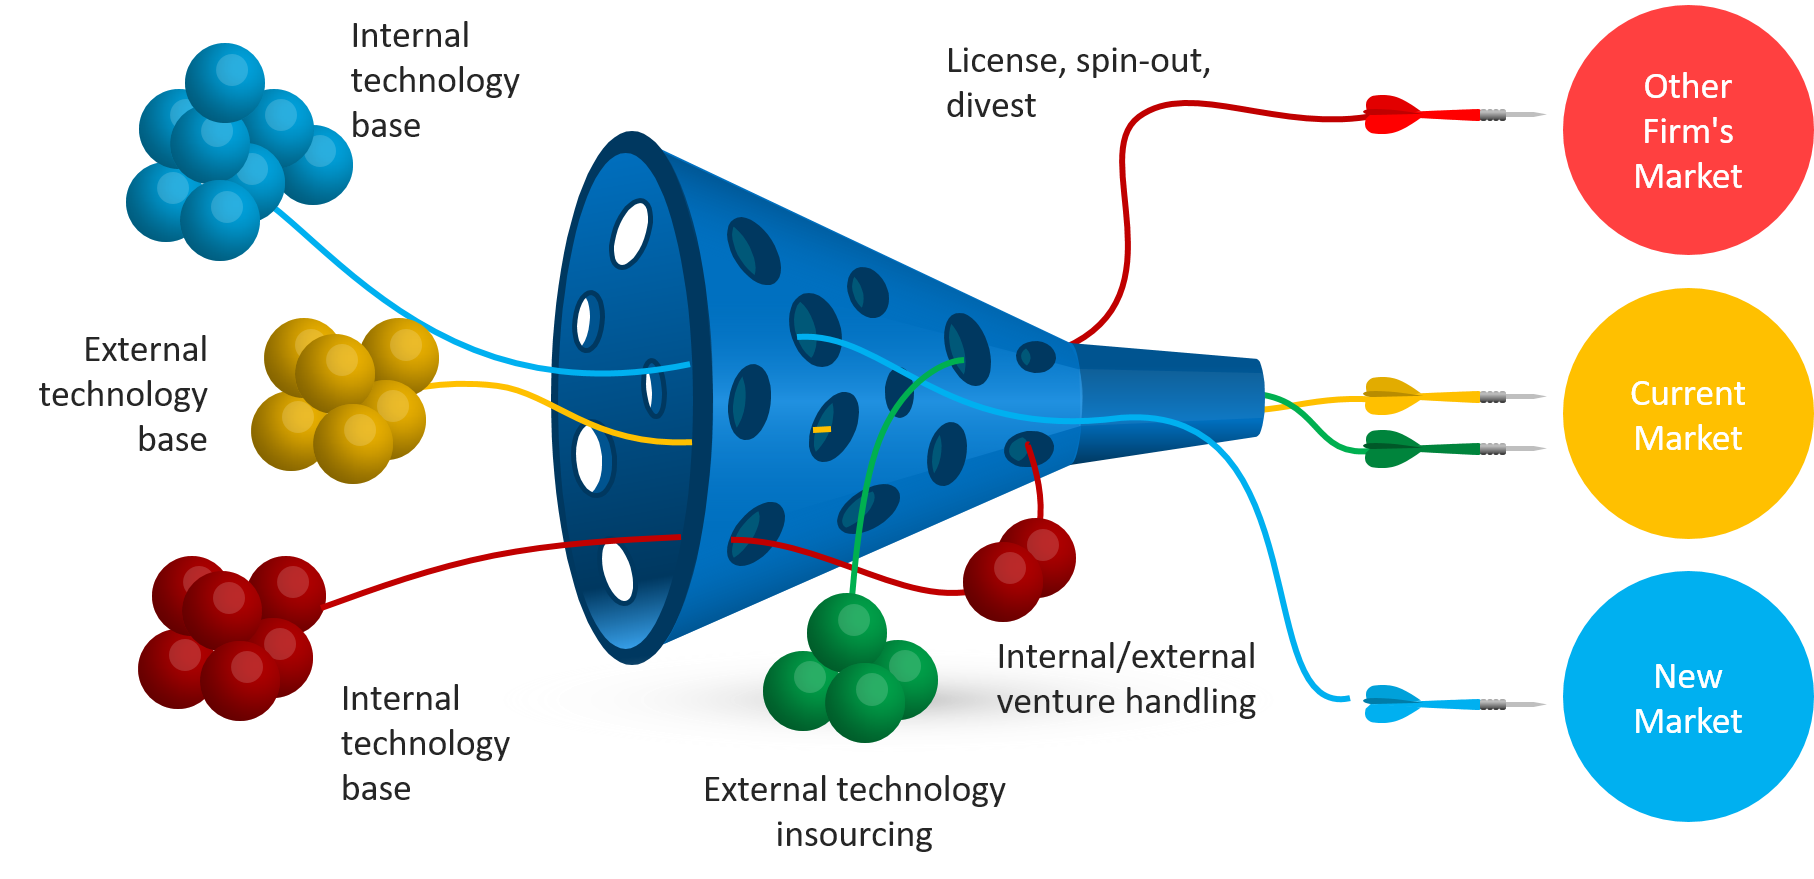
\includegraphics[width=0.9\linewidth]{Images/oi_process_2}
	\caption{Open innovation processes \citep{chesbrough2004open}. Image from SlideModel.}.
	\label{fig:oi_process}
\end{figure}

\subsection{Challenges of open innovation}

Open innovation presents firms with considerable management challenges \citep{hossain2013open,vanhaverbeke2014surfing}. Notable challenges include transforming the existing business model to support open innovation, changing internal approaches to research and development, building a more open culture, finding suitable organisations to partner with, and managing intellectual property \citep{dahlander2010open,sieg2010managerial,lichtenthaler2011your,durst2013success,roper2013externalities,aloini2016structured}. Bridging cognitive gaps between open innovation partners is especially challenging \citep{vanhaverbeke2007connecting,lakemond2016match}. \medskip

\subsubsection{Relative differences in absorptive capacity}

Firms need absorptive capacity to bridge cognitive gaps and allow them to capture value from open innovation \citep{vanhaverbeke2007connecting}. Absorptive capacity is defined as the \enquote{ability of a firm to recognise the value of new, external information, assimilate it, and apply it to commercial ends} \citep{cohen1990absorptive}. Relative differences in absorptive capacity between partner firms can impede the flow of knowledge across firm boundaries, contribute to power imbalances, undermine alliance performance, all of which can result in less favourable open innovation outcomes \citep{szulanski1996exploring,lane1998relative,nooteboom2000learning,vanhaverbeke2007connecting,easterby2008absorptive,phelps2012knowledge} \medskip.
 
Despite the vast body of research that has examined the multidimensional nature of absorptive capacity, the concept remains elusive for both researchers and practitioners \citep{duchek2013capturing,omidvar2013revisiting}. Early conceptualisations of absorptive capacity emphasised the importance of prior related knowledge to facilitate associative learning \citep{cohen1990absorptive}. More recent conceptualisations treat absorptive capacity as a dynamic capability that integrates processes for acquiring, assimilating, transforming, exploiting new knowledge \citep{zahra2002absorptive,todorova2007absorptive,volberda2010perspective,lewin2011microfoundations,marabelli2014knowing}. \medskip

Building absorptive capacity to facilitate open innovation is challenging because it cuts across multiple levels and is contingent not only on social mechanisms for integrating diverse knowledge, but also on the strength or weakness of appropriability regimes \footnote{The term "appropriability regime" describes the ease of imitation. This is a function both of the ease of replication and the efficacy of intellectual property rights as a barrier to imitation. Appropriability is strong when a technology is both inherently difficult to replicate and the intellectual property system provides legal barriers to imitation. When it is inherently easy to replicate and intellectual property protection is either unavailable or ineffectual, then appropriability is weak \citep{teece1998capturing}.} and nature of power-relations \citep{todorova2007absorptive,easterby2008absorptive,duchek2013capturing}. \medskip 

\subsubsection{Communicating tacit knowledge}

Past studies of absorptive capacity have emphasised the importance of prior knowledge possessed by individuals and groups. Most of these studies have treated knowledge as quite explicit, something that can be acquired, stored, processed, and retrieved \citep{omidvar2013revisiting,marabelli2014knowing}. In reality, much of the prior knowledge is tacit, held either in people's minds or in the form of unwritten rules or practices that guide the collective action of groups \citep{mowery1996strategic,leonard1998role,horvath2000working,burt2007secondhand,nonaka2009perspective,goksel2016can,lichtenthaler2016absorptive}. \medskip

Knowledge should not be treated as either tacit or explicit. Rather, knowledge exists on a spectrum where at one end, it is almost completely tacit, embodied in the minds and experience of people. At the other end of the spectrum, knowledge is almost completely explicit, existing in codified or structured form and accessible tip of the iceberg, easy to recognise and access. The vast bulk of the iceberg hidden beneath the surface so other people \citep{polanyi1966tacit,leonard1998role,nonaka2009perspective}. Tacit knowledge tends to be associated with terms such as \enquote{intuition}, \enquote{skill}, \enquote{know-how}, and \enquote{expertise} used to describe knowledge that refers to an ability to perform work \citep{mcadam2007exploring}. \medskip

Much knowledge often remains tacit for various reasons. One reason is that individuals may be reluctant to surrender any advantages their tacit knowledge or know-how affords them. Another reason is that people are either unaware of the tacit dimension of their knowledge or unable to express what they know \citep{leonard1998role,eraut2000non}. Tacit knowledge is also prone to being discounted or misunderstood by others \citep{burt2007secondhand}. Because it is largely invisible, tacit knowledge is a tremendous source of competitive advantage \citep{nelson1982evolutionary,barney1991firm,grant1996toward,smith2001role,chilton2007dimensions,lu2015job}. Note that knowledge should not be treated as either tacit or explicit. Rather, knowledge exists on a spectrum where at one end, it is almost completely tacit, embodied in the minds and experience of people. At the other end of the spectrum, knowledge is almost completely explicit, existing in codified or structured form and accessible to other people \citep{polanyi1966tacit,leonard1998role,nonaka2009perspective}. \medskip

The leading edge of the firm’s learning, and often the source of its future innovations, tends to be found in the tacit knowledge of its people \citep{horvath2000working}. Tacit knowledge guides the thought processes that produce novel ideas \citep{leonard1998role,amar2008descriptive,seidler2008use}. Tacit knowledge tends to be associated with terms such as \enquote{intuition}, \enquote{skill}, \enquote{know-how}, and \enquote{expertise} used to describe knowledge that refers to an ability to perform work \citep{mcadam2007exploring}. The most common application of tacit knowledge is problem-solving. People with expertise borne from experience not only are able to recognise the situation in which they find themselves in, but also know which actions might be appropriate for dealing with it \citep{simon1971human,leonard1998role}. Tacit knowledge can also be used to reformulate problems by viewing these differently in intuitive ways \citep{leonard1998role}. \medskip

Much knowledge often remains tacit for various reasons. One reason is that people are either unaware of the tacit dimension of their knowledge or unable to express what they know. Individuals may also be reluctant to give up any advantages their tacit knowledge or know-how affords them \citep{leonard1998role,eraut2000non}. `````````````````````````````````````````````````````````````````Tacit knowledge is prone to being discounted or misunderstood by others \citep{burt2007secondhnd mobilising tacit knowledg facilihe transfer of explicit knowledge. Without tacit knowledge, explicit knowledge quickly loses its meaning \citep{seidler2008useis unavailable for conscious inspection, it can only be assessed using indirect approaches \citep{chilton2007dimensions}.                                                                                                                                                                                                                                                                                                                      n processes, namely \enquotemph{socialisation}, \enquotemph{externalisation}, \enquotemph{combination}, and \enquotemph{internalisation}. The process of \emph{socialisation} aims to create common understanding through shared experiences and the demonstration of technical skills. \emph{Externalisation} is the process of expressing and articulating knowledge through using metaphors, models and analogies. \emph{Combination} organises concepts into a knowledge system whereas \emph{internalisation} embodies knowledge through \enquote{learning by doing}. The relative efficiency in knowledge conversion is what gives the firm rent \citep{nonaka1994dynamic,nonaka1995knowledge}. \medskip



The management challenge is getting others to fully appreciate tacit knowledge held in people's minds or group practice.  


This emphasises the need for people in boundary spanning roles to aid the transfer of diverse and often complex knowledge \citep{tushman1981boundary,allen1984managing,szulanski2003sticky,seidler2008use,meyer2010rise,chesbrough2012open}. \medskip

\subsubsection{Brokering productive relationships}

Boundary spanners play a key role in open innovation as they facilitate the translation, integration and combination of unfamiliar and distant knowledge \citep{tushman1981boundary,allen1984managing,,meyer2010rise,chesbrough2012open}. They also broker new relations between otherwise disconnected actors in different organisational networks \citep{granovetter1973strength,burt2004structural,burt2007secondhand}. \medskip

Management efforts to create or widen existing inter-organisational networks may be frustrated by people reluctant to form new ties, facilitate third-party ties, or otherwise change their existing networks \citep{davis2010agency}. Not-invented-here and not-shared-here (also referred to as not-sold-here) syndromes can also stymie knowledge exchange \citep{lichtenthaler2006attitudes,lichtenthaler2011your,de2014neither,podmetina2015skills,chesbrough2017future}. Not-invented-here syndrome refers to resistance within a firm against externally developed knowledge \citep{katz1982investigating,hussinger2011search,antons2015opening}. Not-shared-here syndrome is a negative attitude towards external exploitation of internally developed knowledge \citep{chesbrough2003open,lichtenthaler2006attitudes,de2014neither}. Figuring out ways to overcome negative attitudes towards knowledge sharing is essential to allow the formation of new productive relationships that enable knowledge to be recombined in unique and valuable ways \citep{uzzi1997social,nahapiet1998social,obstfeld2005social,lane2006reification,davis2010agency,meyer2010rise}.\medskip

\section{Research opportunity}

Quantitative measures fail to capture the complex and dynamic nature of absorptive capacity \citep{easterby2008absorptive,duchek2013capturing}. Recent studies point to a practice-based approach as most appropriate for identifying the routines and practices that build absorptive capacity \citep[e.g.][]{duchek2013capturing,omidvar2013revisiting,marabelli2012knowledge,marabelli2014knowing}. Unless acted upon, tacit and explicit knowledge is simply a latent resource. Knowledge becomes valuable when enacted in practice, symbolising the very act of knowing \citep{cook1999bridging,duguid2005art,marabelli2014knowing,freeman2015knowledge}. 


The extent to which tacit knowledge helps bridge cognitive gaps is poorly understood. Research into brokerage of tacit knowledge is also lacking. This is hardly surprising, given tacit knowledge is difficult to characterise let alone measure \citep{zander1995knowledge,cavusgil2003tacit}. 
There is little doubt that tacit knowledge has a significant influence on a firm's absorptive and innovative capacity, and warrants much more attention than it has received so far.  
\medskip

 Given much knowledge is held either in people's minds or in the form of unwritten rules or practices that guide the collective action of groups, a practice-based approach makes a lot of sense.

\medskip


\subsection{Exploring motivational factors}

Managing the flow of tacit knowledge across organisational boundaries is confounded by the fact that tacit knowledge sharing cannot be mandated but happens through volition or free will \citep{polanyi1966tacit}. Moreover, tacit knowledge can only be shared through direct observation, either via face-to-face social interaction or by video demonstrations \citep{haldin2000difficulties,koskinen2003tacit}. Tacit knowledge is not something that is transferred. Rather, tacit knowledge is interpreted within a specific context. Face-to-face social interaction is considered the richest medium because it allows immediate feedback to check understanding and correct interpretations \citep{koskinen2003tacit}. \medskip

Since tacit knowledge requires significant effort to communicate, people need to be sufficiently motivated to seek out or share tacit knowledge \citep{leonard1998role}. Past studies show a significant and positive relation between an individual's level of intrinsic motivation and the amount of tacit knowledge they share \citep[e.g.][]{osterloh2000motivation,kaser2001knowledge,smith2001role}. While these studies highlight the importance of individual motivation, the social processes underpinning tacit knowledge sharing and how this impacts open innovation are not well understood. 


There is a need to research how individual motivation shapes knowledge sharing relations

\medskip

\subsubsection{Unpacking power-relations}

Whereas many claim \enquote{knowledge is power}, not much attention has been given to power and power-relations in the knowledge management literature \citep{heizmann2015power}. The current power literature is dominated by two contrasting views of power, namely \enquote{power as domination}, also referred to as \enquote{power-over}, and \enquote{power as empowerment}, often characterised as \enquote{power-to} \citep{haugaard2012rethinking}. Sharing know-how or expertise (i.e. tacit knowledge) is all about empowering others so they can perform work more independently and confidently. \medskip

The network perspective treats power as inherently relational \citep{ibarra1993network}. Power arises from occupying advantageous positions in networks of social relations. How an actor is embedded in a social network either imposes constraints on the actor or presents the actor with opportunities. Essentially, actors with fewer constraints and more opportunities occupy favourable structural positions. Being in a favoured position means that an actor may extract better bargains in exchanges, have greater influence, and be a focus for deference and attention from those in less favoured positions \citep{burt1992structural,hanneman2005introduction,simpson2011network}. \medskip

\citet{obstfeld2014brokerage} define brokerage as \enquote{behaviour by which an actor influences, manages, or facilitates interactions between other actors}. This definition allows brokerage to be seen in terms of \enquote{power-over} and \enquote{power-to}. \citet{obstfeld2014brokerage} describe three strategic orientations to brokerage: \emph{conduit brokerage} is about a third-party who transfers information, knowledge, or other resources between two disconnected parties. The broker mediates rather than moderates the relationship between two others and may help them synthesise new knowledge. With \emph{tertius gaudens brokerage}, the broker aims to exploit differences between two parties by either keeping them apart or playing one against another. In contrast, \emph{tertius iungens brokerage} is about a third-party who introduces two otherwise disconnected parties to each other and encourages them to collaborate (Figure \ref{brokerage}). \medskip 

\begin{table}[]
\small
\centering
\caption{Three forms of brokerage process. Reproduced from \citet{obstfeld2014brokerage}.}
\label{brokerage}
\begin{tabularx}{\textwidth}{p{3.5cm}p{3.5cm}p{3.5cm}p{3.5cm}}
	\toprule
	& \multicolumn{1}{c}{Conduit} & \multicolumn{1}{c}{Tertius Gaudens} & \multicolumn{1}{c}{Tertius Iungens} \\ \midrule
	& \begin{minipage}{.2\textwidth} \centering 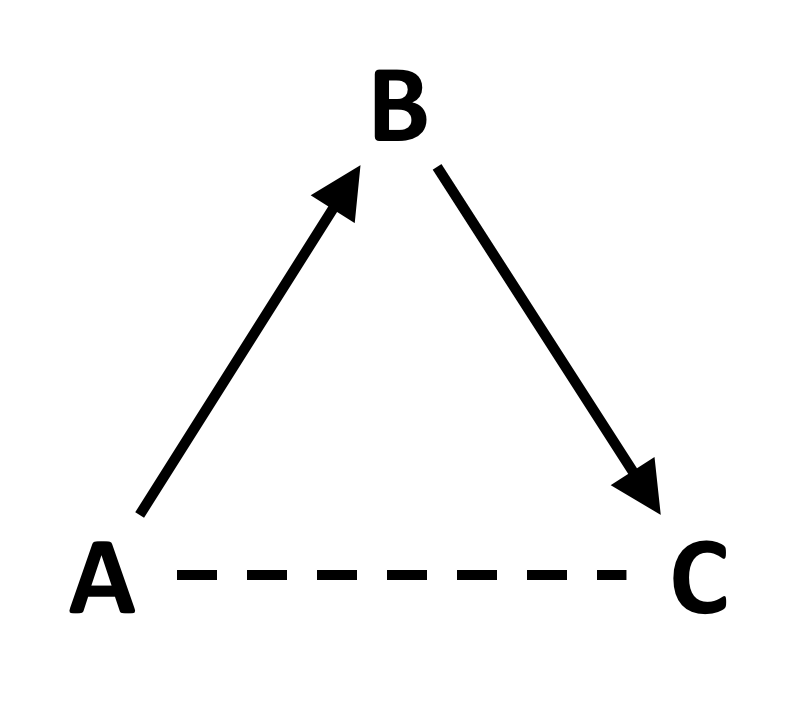
\includegraphics[width=0.7\linewidth]{Images/CDT_brokerage} \end{minipage}  & \begin{minipage}{.2\textwidth} \centering 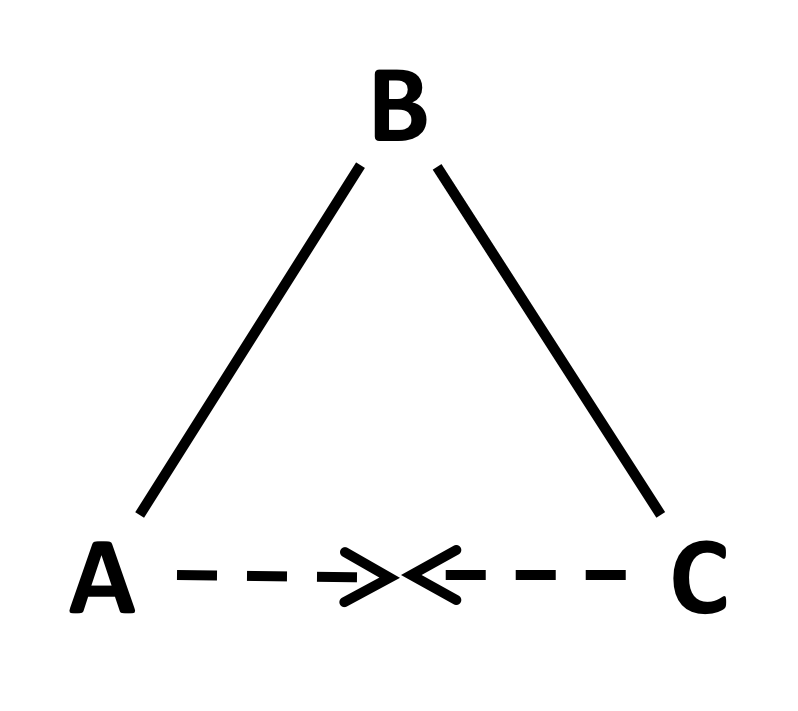
\includegraphics[width=0.7\linewidth]{Images/TG_brokerage_1} \end{minipage}  & \begin{minipage}{.2\textwidth} \centering 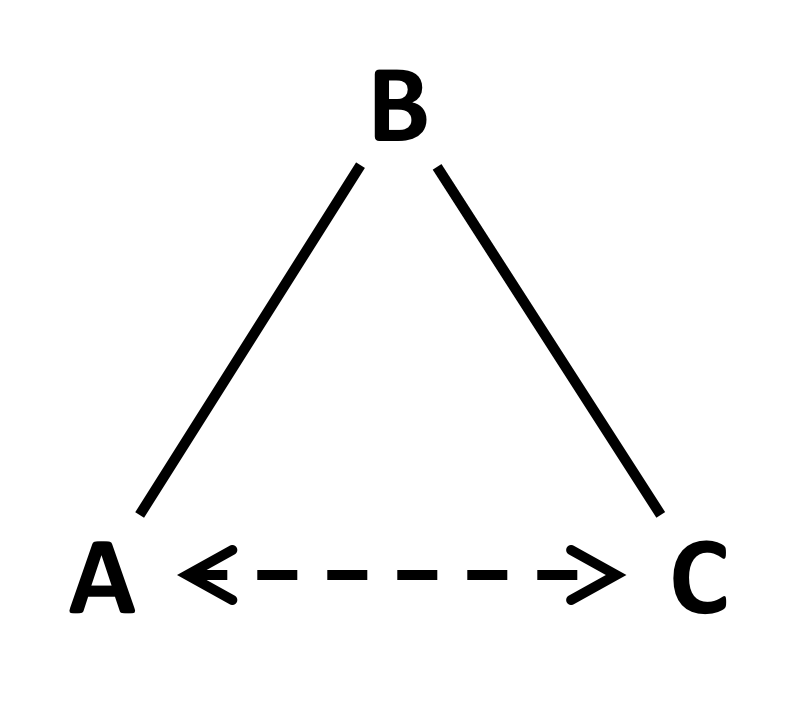
\includegraphics[width=0.7\linewidth]{Images/TI_brokerage} \end{minipage}   \\
	&  & \begin{minipage}{.2\textwidth} \centering 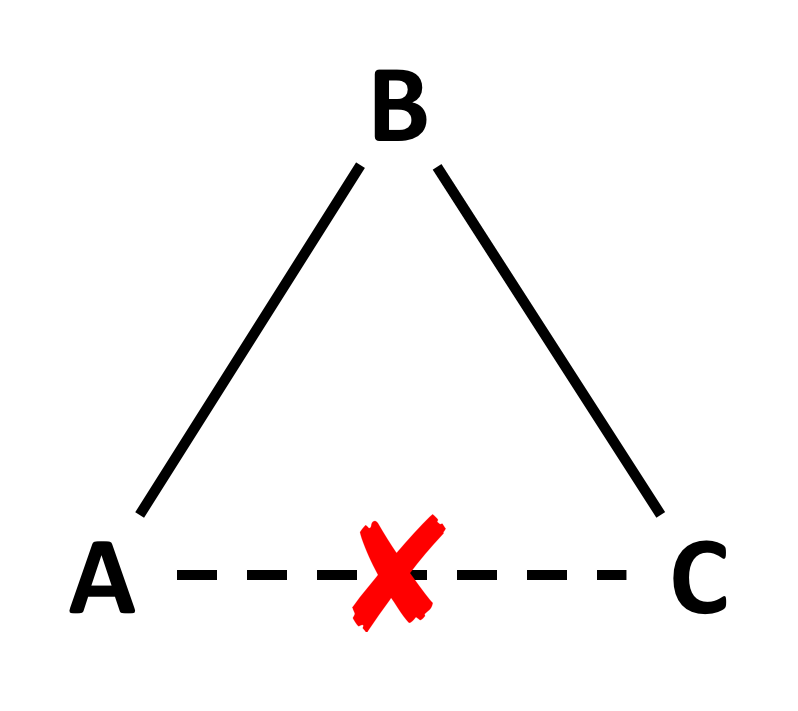
\includegraphics[width=0.7\linewidth]{Images/TG_brokerage_2} \end{minipage}  &  \\ \midrule
	Open network\\(absence of A-C tie) & B transfers information, knowledge, or other resources between A and C where A and C have no prospect of meeting & B plays A and C against one another or keeps A and C apart & B introduces A and C where A and C have no prior tie \\ \midrule
	Closed Network\\(presence of A-C tie) & B facilitates transfer between A and C and may help synthesize new knowledge & B cultivates conflict,,competition, or separation between A and C (divide et impera) & B coordinates new collaborative action between A and C \\ \bottomrule
\end{tabularx}
\end{table}

From an open innovation perspective, \emph{tertius iungens brokerage} is quite important, especially in the early stages of collaboration, when many actors do not know fellow collaborators in partner organisations. Not only that, knowledge held by third parties is also likely to be unfamiliar. Once ties have been established through \emph{tertius iungens brokerage}, \emph{conduit brokerage} is needed to help synthesise and transform knowledge into novel ideas \citep{fleming2007collaborative,lingo2010nexus,quintane2016brokers}. \citet{gould1989structures} describe \emph{conduit brokerage} in terms of \emph{coordination}, \emph{liaison}, \emph{itinerant}, \emph{representative}, and \emph{gatekeeper} roles (Figure \ref{gf_params}). Each role expresses a different power dynamic and one should be to use the relative proportion of each role to characterise power-relations in open innovation collaborations. A better understanding of power-relations can contribute to more effective management interventions. 

\begin{table}[]
	\small
	\centering
	\caption{Gould-Fernandez brokerage roles}
	\label{gf_params}
	\begin{tabularx}{\textwidth}{@{}lcl@{}}
		\toprule
		\multicolumn{1}{c}{Role} & \multicolumn{1}{c}{Graphic} & \multicolumn{1}{c}{Explanation} \\ \midrule
		b\textsubscript{O} (liaison role)			&  \begin{minipage}{.2\textwidth} \centering 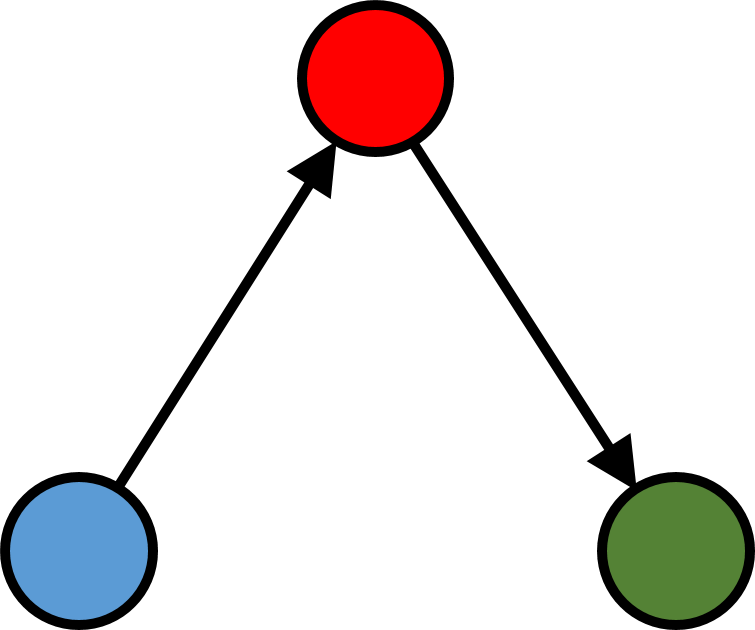
\includegraphics[width=0.4\linewidth]{Images/b_O} \end{minipage}	& \begin{tabular}[c]{l}Broker mediates contact between two\\ individuals from different groups,\\ neither of which is the group to\\ which he or she belongs.\end{tabular}\\ [10ex]
		b\textsubscript{IO} (representative role)	& \begin{minipage}{.2\textwidth} \centering 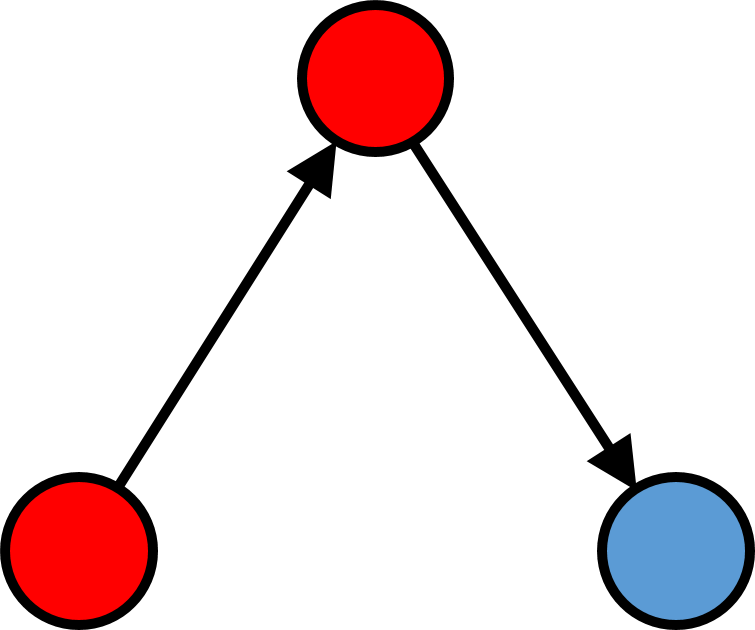
\includegraphics[width=0.4\linewidth]{Images/b_IO} \end{minipage}   & \begin{tabular}[c]{l}Broker mediates an outgoing contact\\ from an in-group member to an\\ out-group member.\end{tabular}\\ [10ex]
		b\textsubscript{OI} (gatekeeper role)		& \begin{minipage}{.2\textwidth} \centering 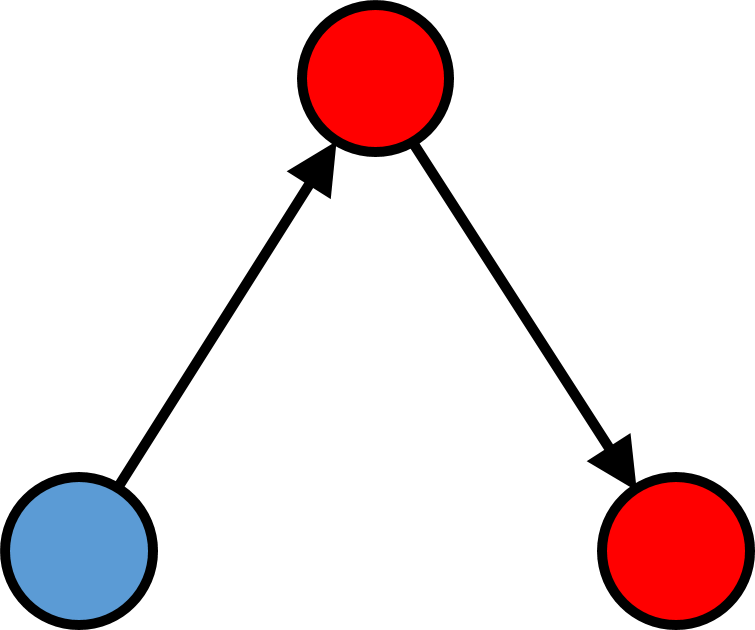
\includegraphics[width=0.4\linewidth]{Images/b_OI} \end{minipage}   & \begin{tabular}[c]{l}Broker mediates an incoming contact\\ from an out-group member to an\\ in-group member. \end{tabular}\\ [10ex]
		w\textsubscript{O} (itinerant broker)		&  \begin{minipage}{.2\textwidth} \centering 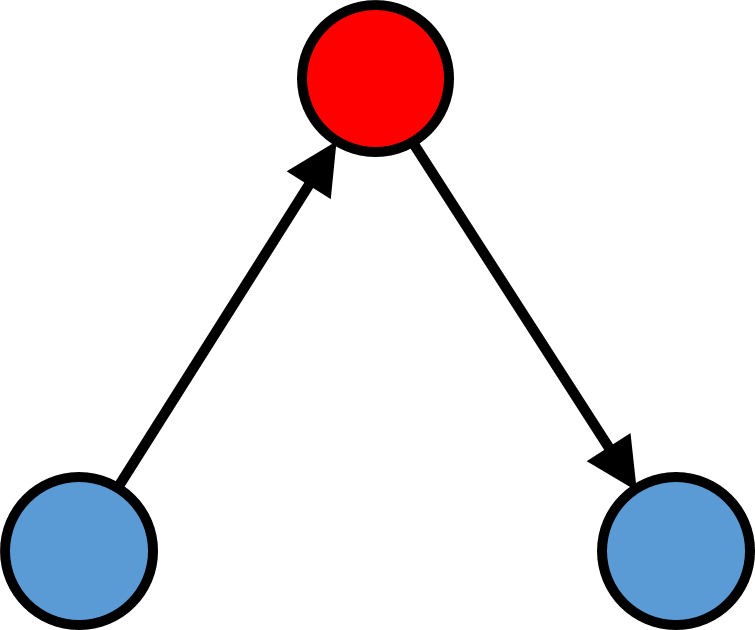
\includegraphics[width=0.4\linewidth]{Images/w_O} \end{minipage}   & \begin{tabular}[c]{l}Broker mediates contact between two\\ individuals from a single group to\\ which he or she does not belong. \end{tabular}\\ [10ex]
		w\textsubscript{I} (coordination role)		& \begin{minipage}{.2\textwidth} \centering 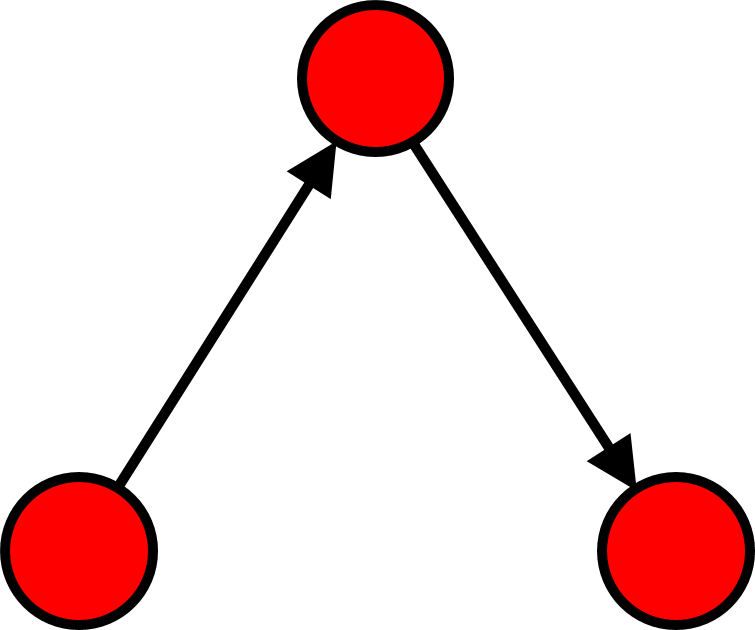
\includegraphics[width=0.4\linewidth]{Images/w_I} \end{minipage}    & \begin{tabular}[c]{l}Broker mediates contact between two\\ individuals from his or her own\\ group. \end{tabular}\\ 
		\bottomrule
	\end{tabularx}
\end{table}
 





Mixed method social network analysis presents an opportunity to assess how knowledge is enacted in practice and what this means in terms of building absorptive capacity and deleivering successful open innovation outcomes. \medskip 

\section{Study objectives}

Innovation is a socially intensive process that involves creative individuals who share knowledge and co-create ideas within a group \citep{leonard1998role}. Converting external knowledge into valuable innovations is largely dependent on the configuration of knowledge sharing and idea-generation networks \citep{tortoriello2010activating}. Little is known about the social practices that build absorptive capacity and how these are affected by tacit knowledge \citep{tortoriello2015social,lichtenthaler2016absorptive}. The aim of social network analysis is detecting and interpreting patterns of social ties between actors \citep{de2011exploratory}. We can use social-network analysis to investigate the connection between individual positions in knowledge sharing and idea-generation networks with open-innovation outcomes, and assess how power-relations affect knowledge-sharing behaviour \citep{van2010use,marabelli2014knowing}. \medskip

There is a limit to what social-network analysis can tell us about social practices. New knowledge tends to be generated within a particular context, such as a product of observation or rich interactions that help individuals think about problems and solutions in a new context \citep{nonaka1994dynamic,wenger2000communities,cross2015investing}. Social network analysis needs to be complemented by a qualitative study to capture the context in which knowledge sharing and idea generation occurs. \medskip 

This study employs mixed methods social network analysis to assess absorptive capacity processes within three open-innovation collaborations. Attention is focussed on psychological and social factors that govern knowledge-sharing behaviour and how these might influence tacit-knowledge exchange. \medskip

The overarching research question in this study is \enquote{how do psychological and social factors shape the development of absorptive capacity in open innovation?}. This question is answered by addressing three sub-questions:\medskip

\begin{enumerate}
	\item To what extent does autonomous motivation predict knowledge sharing behaviour? How is this affected by the level of tacit knowledge being exchanged?
	\item How do patterns of brokerage differ according to the level of tacit knowledge being shared? What does this reveal about the nature of the collaboration, and what does this tell us about power-relations?
	\item To what extent does the level of tacit knowledge exchange predict the emergence of novel ideas, and what does this reveal about the complexity of the innovation challenge? 
\end{enumerate}

The mixed methods social network analysis uses statistical modelling to assess how individual attributes, such as level of personal motivation, educational background, and work experience, influence the emergence of knowledge-sharing connections. The modelling also exposes patterns of social interaction operating across multiple levels \citep{monge2003theories,lusher2012exponential}. The modelling is complemented by semi-structured interviews that capture the industrial, organisational, and cultural contexts governing the emergence of collaborative social structures.\medskip 

\section{Research contribution}

This study advances knowledge in two ways. Firstly, the study provides fresh insight into how tacit knowledge shapes absorptive capacity and contributes to the success of open innovation. Secondly, it tests the feasibility of using social-network analysis to assess how absorptive capacity emerges in practice. Such analysis offers some advantages over a practice-based approach based on ethnography in terms of objectivity, generalisability, and time. By highlighting key social mechanisms that build absorptive capacity in collaborative innovation, this study contributes to more effective and practical ways to create and capture value from inter-organisational relationships.\medskip

\section{Document structure}

This document is organised into ten chapters. Chapter Two explains how the concept of absorptive capacity has evolved into a dynamic capability encompassing cognitive and behavioural change. This suggests that any assessment of absorptive capacity needs to consider what factors contribute to cognitive and behavioural change. \medskip

Chapter Three explains what social networks are and introduces key psychological and social theories that can be used to assess knowledge sharing behaviour. The mixed method research methodology used in this study is presented in Chapter Four. This includes a detailed description of the multi-theoretical multilevel-analytical framework used to assess the dynamic nature of absorptive capacity. \medskip

Chapter Five highlights the distinguishing characteristics of the three open-innovation case studies. Results from the mixed method social network analysis are presented separately for each case in Chapters Six, Seven, and Eight. Comparisons between the three sets of results are discussed in Chapter Nine. \medskip 

Finally, Chapter Ten summarises the key findings of this study and reflects on some key lessons learned as this study unfolded. 